\chapter{ Аналитический раздел}
\label{cha:analytical}
    В данном разделе будут рассмотрены основные теоритические понятия алгоритма 
    обратной трассировки лучей.

    \section{Алгоритм обратной трассировки лучей}
	Методы трассировки лучей на сегодняшний день считаются наиболее мощными методами создания реалистических изображений. Универсальность методов трассировки в значительной степени обусловлена тем, что в их основе лежат простые и ясные понятия, отражающие наш опыт восприятия окружающего мира.

	Метод обратной трассировки лучей позволяет значительно сократить перебор световых лучей по сравнению с классической трассировкой. В нем отслеживаются лучи не от источников, а из камеры. Таким образом, трассируется определенное число лучей, равное разрешению картинки.

	Предположим, что у нас есть камера и экран, находящийся на расстоянии d от нее (рисунок \ref{png:axis}).

        \begin{figure}[h!]
            \centering
            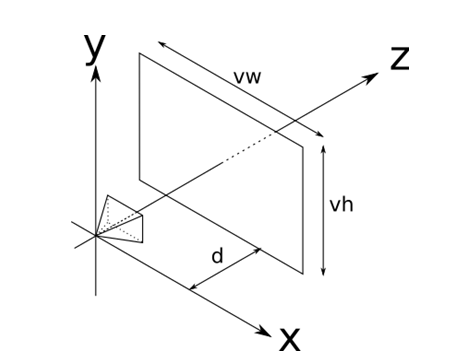
\includegraphics[scale=0.6]{axis.png}
	 \caption{Расположение камеры и сцены}
            \label{png:axis}
        \end{figure} 

 Разобьем экран на квадратики. Дальше будем по очереди проводить лучи из камеры в центр каждого квадратика (первичные лучи). Найдем пересечение каждого такого луча с объектами сцены и выберем среди всех пересечений самое близкое к камере. Далее, применив нужную модель освещения, можно получить изображение сцены.

	Но можно пойти дальше. Если мы хотим смоделировать такое явление, как отражение, нам необходимо из самого близкого пересечения пустить вторичные лучи. Например, если поверхность отражает свет и она идеально ровная, то необходимо отразить первичный луч от поверхности и пустить по этому направлению вторичный луч. 






\newpage